% !TeX root = ../main.tex
% Add the above to each chapter to make compiling the PDF easier in some editors.
\usetikzlibrary{positioning,fit,calc,arrows,shapes}

\chapter{Background}\label{chapter:background}

\section{Active Monitoring and Black Box Monitoring}

Monitoring IT systems brings insight into systems in terms of observability, becoming increasingly critical to improving systems. Based on simulation data generated synthetically, active monitoring proactively monitors the performance of networks, applications, and infrastructure~\parencite{splunkActiveVsPassive2023}. Another well-known monitoring method is black box monitoring. Like active monitoring, black box monitoring evaluates a system's functionality based on its responses to given inputs while abstracting away the system's internal workings~\parencite{jorgensenSoftwareTestingCraftsman2021}. 

Active monitoring, also called synthetic monitoring, mainly identifies potential application issues, including health checks, \ac{API} endpoint tests, etc. In addition, active monitoring also includes evaluating the performance of hardware resources and benchmarking the network performance~\parencite{splunkActiveVsPassive2023}. For example, the \ac{QoS} requirements of the network like latency and bandwidth, the ~\ac{CPU} utilization, and the memory utilization. 

Black box monitoring is a well-established approach to system analysis, commonly applied in software testing and network monitoring. In contrast to white box monitoring, which baesd on metrics exposed by the internals of the system, it focuses on external behavior rather than internal metrics~\parencite{beyerSiteReliabilityEngineering2016}. This technique metaphorically views the system as a "black box" in ~\autoref{fig:black-box-monitoring-illustration}, signifying that the internal mechanisms are not visible or accounted for in the evaluation process~\parencite{myersArtSoftwareTesting2004}. 

\begin{figure}[htpb]
    \centering
    % This should probably go into a file in figures/
    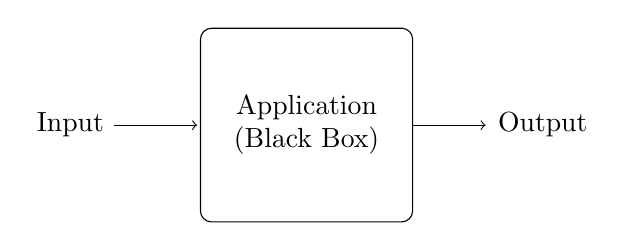
\begin{tikzpicture}[shorten >=1pt, node distance=3cm, auto]
      \node (R0) {Input};
      \node (R1) [right of=R0, minimum height=7em, text width=7em, align=center, draw, rounded corners] {Application\\(Black\ Box)};
      \node (R2) [right of=R1] {Output};
      \path[->]
        (R0) edge node {} (R1)
        (R1) edge node {} (R2);
    \end{tikzpicture}
    \caption[Black Box Monitoring Illustration]{An illustration of the Black Box Monitoring.}\label{fig:black-box-monitoring-illustration}
\end{figure}

Active monitoring and black box monitoring share some similar features but embody distinct concepts. Both involve simulating requests to target \ac{API}s or other endpoints, such as those of \ac{TCP}, \ac{HTTP}, or other customized protocols. Specifically, These symptom-oriented techniques mimic user behavior, thereby reflecting real issues~\parencite{beyerSiteReliabilityEngineering2016}. By definition, active monitoring can encompass black box monitoring but focuses on different aspects. Active monitoring emphasizes proactive check-ups, actively testing and querying systems, while black box monitoring is more of an observational approach, focusing on the outcomes and behaviors of systems without delving into their internal mechanics. In summary, despite of slight difference, both methods are valuable in system monitoring and could contribute to the comprehensive view of system health and performance. 

In system monitoring, the "Four Golden Signals" are essential: Latency, Traffic, Errors, and Saturation. Latency signifies response times, differentiating between successful and failed requests. Traffic gauges demand, such as \ac{HTTP} requests per second. Errors identify the rate of failures, whether explicit, implicit, or policy-driven. Saturation looks at resource utilization and potential bottlenecks~\parencite{beyerSiteReliabilityEngineering2016}. Bridging these metrics, active monitoring proactively tests systems for performance and reliability, while black box monitoring observes system behavior without internal visibility. The combination enhanced the effectiveness of the "Four Golden Signals," ensuring comprehensive system monitoring and optimal system performance.

As the IT landscape becomes more complex with microservices and cloud-based applications, understanding the internals of every service can be overwhelming. In such a scenario, active monitoring and black box monitoring's ability to provide a holistic view of system behavior can be highly beneficial. Moreover, in light of growing privacy regulations and data protection measures, the non-invasive approach aligns with the current trends. Simulating test inputs and focusing on system outputs rather than internals could minimize privacy or data protection concerns. 

In conclusion, active monitoring and black box monitoring are vital tools for system testing and monitoring. Its future appears increasingly integrated with cloud technologies and aligned with user-centric design principles. Nevertheless, they should not be considered a stand-alone solution but rather a component of a comprehensive monitoring strategy that incorporates various techniques to manage system performance effectively. 

\section{Prometheus Agent and Blackbox Exporter}

The renowned Prometheus ecosystem provides two important components: the Prometheus Agent and the Blackbox Exporter. These technologies are extensively employed in various enterprises for monitoring applications in testing and production environments. Their widespread adoption is a testament to the reliability and robustness of the Prometheus platform in handling diverse monitoring needs.

The Prometheus Agent is a specialized mode of a standard Prometheus instance aimed at efficient data scraping and remote write as in ~\autoref{fig:prometheus-agent}. Unlike a full-fledged Prometheus server with functionalities like data storage and querying, the Prometheus Agent is simplified for specific tasks, making it an ideal choice in distributed systems where resource optimization is crucial. This mode is invaluable when a full Prometheus server setup is unnecessary, facilitating a more resource-efficient deployment. It is particularly effective in large-scale environments where managing the overhead and complexity of multiple complete Prometheus instances would be impractical~\parencite{prometheusIntroducingPrometheusAgent}.

\begin{figure}[htpb]
    \centering
    % This should probably go into a file in figures/
    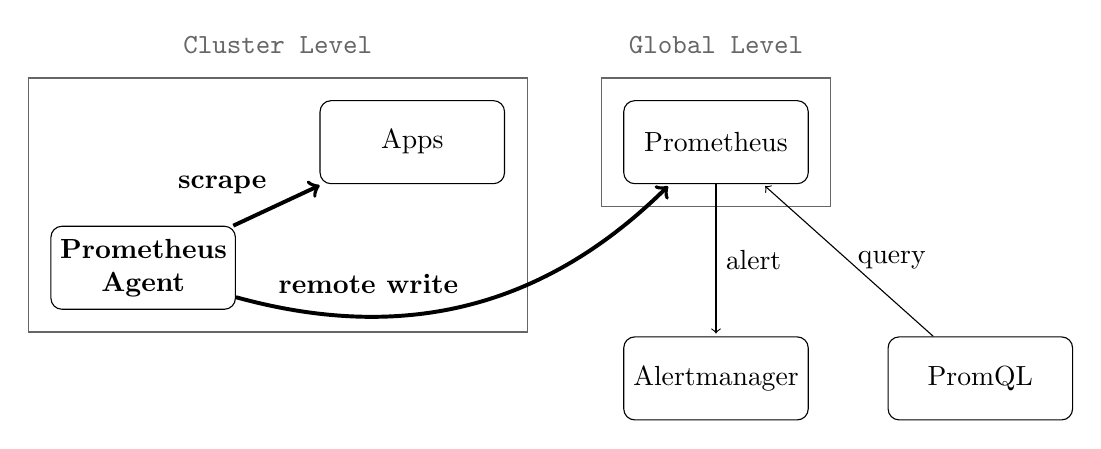
\begin{tikzpicture}[
        shorten >=1pt,
        zonetag/.style={align=center, font=\fontsize{10}{10}\color{black!60}\ttfamily},
        node/.style={draw, align=center, minimum height=3em, anchor=west, rounded corners}, 
        zone/.style={draw=black!60, inner sep=8pt}
      ]

      \node (PA) [node distance=1cm, text width=6em, node, font=\bfseries] {Prometheus\\Agent};
      \node (Apps) [node distance=1.5cm, above right=of PA, text width=6em, node] {Apps};
      \node (CZ) [zone, fit={(PA) (Apps)}] {};
      \node (C) [zonetag, node distance=0.5em, above=of CZ] {Cluster Level};

      \node (P) [node distance=1.5cm, right=of Apps, text width=6em, node] {Prometheus};
      \node (Am) [node distance=3cm, below=of P.west, text width=6em, node] {Alertmanager};
      \node (PQ) [node distance=1cm, right=of Am, text width=6em, node] {PromQL};
      \node (GZ) [zone, fit={(P)}] {};
      \node (G) [zonetag, node distance=0.5em, above=of GZ] {Global Level};
  
      \path[->] (P) edge node[auto] {alert} (Am);
      \path[->] (PA) edge[bend right, line width=0.5mm] node[auto, font=\bfseries] {remote write} (P);
      \path[->] (PA) edge[line width=0.5mm] node[auto, font=\bfseries] {scrape} (Apps);
      \path[->] (PQ) edge node[auto, right] {query} (P);

    \end{tikzpicture}
    \caption[Prometheus Agent with Scrape and Remote Write]{Prometheus Agent with Scrape and Remote Write.}\label{fig:prometheus-agent}
\end{figure}

The Blackbox Exporter, an essential element of the Prometheus toolkit, is designed to probe external endpoints across multiple protocols, including \ac{HTTP}/\ac{HTTPS}, \ac{TCP}, and \ac{ICMP}. This capability is fundamental to black box monitoring, enabling the assessment of system health and performance from an external viewpoint without necessitating internal access to the monitored system~\parencite{prometheusBlackboxExporter2023}. The Blackbox Exporter is instrumental in situations where internal monitoring is either not feasible or insufficient, such as in third-party services or in environments where internal metrics are not available or reliable.

Integrating the Prometheus Agent with the Blackbox Exporter fosters a distributed scheduler-executor architecture. This approach allows for a more granular and distributed monitoring framework, which is highly adaptable and can be effectively implemented across various \ac{PaaS} clusters with latencies~\parencite{prometheusUnderstandingUsingMultitarget}. Such an architecture bolsters the scalability and resilience of the monitoring system, rendering it suitable for large-scale and intricate environments. This distributed nature enhances the system's ability to scale and ensures a more resilient monitoring setup capable of withstanding node failures and network partitions~\parencite{prometheusIntroducingPrometheusAgent}.

Achieving optimal availability and scalability with the Prometheus Agent and Blackbox Exporter needs additional configuration and management. For the Prometheus Agent, employing relabeling is a crucial horizontal scaling or sharding strategy~\parencite{prometheusHowRelabelingPrometheus}. This method distributes the workload across multiple Prometheus Agent instances with a hidden label with hashed value, augmenting the system's capacity to handle substantial data volumes efficiently. Regarding the Blackbox Exporter, scalability is further enhanced by integrating a load balancer with properly configured scaling parameters, ensuring an even distribution of the probing load and maintaining system performance, even under high demand~\parencite{prometheusIntroducingPrometheusAgent}.

Overall, the active and extensive community surrounding Prometheus plays a significant role in the continuous improvement and reliability of the Prometheus Agent and Blackbox Exporter. This support ensures consistent updates and maintenance, effectively addressing the evolving needs and challenges in the monitoring domain. However, utilizing the Prometheus Agent and Blackbox Exporter to achieve scalability and manageability requires additional configurations and operations. Consequently, automating the scaling and management operations for both the Prometheus Agent and Blackbox Exporter emerges as a critical issue.

\section{Operator Pattern and Prometheus Operator}

The Operator Pattern, defined by the \ac{CNCF}, represents a paradigm shift in Kubernetes, enabling users to automate the maintenance and configuration of applications~\parencite{kubernetesOperatorPattern}. The Prometheus Operator embodies this pattern, serving as an implementation that addresses the practical needs of deploying and managing Prometheus components. Through reconciliation, the Prometheus Operator aligns the deployment's actual state with the user's desired state, streamlining its lifecycle in Kubernetes~\parencite{prometheusoperatorIntroduction2020}.

The Operator Pattern extends Kubernetes' native capabilities by introducing the \ac{CR} and controllers. The operator, that is, the controller, is the essential software extension that utilizes the Kubernetes control plane and \ac{API} to create, configure, and manage instances of complex stateful applications on behalf of a Kubernetes user~\parencite{dobiesKubernetesOperators}. As shown in ~\autoref{fig:operator-pattern}, the controller continuously reconciles the current state with the desired state, encapsulated in custom resources, using a loop to transition watched objects to their target state. In conclusion, the Operator Pattern encapsulates operational knowledge, automating the management tasks typically requiring manual operations~\parencite{cncfCNCFOperatorWhite}. 

\begin{figure}[htpb]
    \centering
    % This should probably go into a file in figures/
    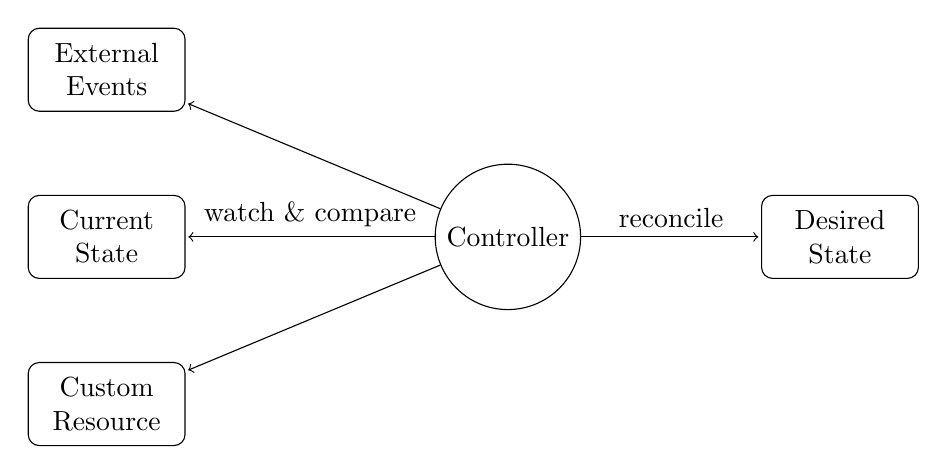
\begin{tikzpicture}[
        shorten >=1pt,
        zonetag/.style={align=center, font=\fontsize{10}{10}\color{black!60}\ttfamily},
        node/.style={draw, align=center, minimum height=3em, rounded corners}, 
        zone/.style={draw=black!60}
      ]

      \node (EE) at(0, 0) [node, text width=5em] {External\ Events};
      \node (CS) [node distance=3em, below=of EE, text width=5em, node] {Current\ State};
      \node (CR) [node distance=3em, below=of CS, text width=5em, node] {Custom\ Resource};
      \node (C) [node distance=9em, right=of CS, circle, node] {Controller};
      \node (DS) [node distance=12em, right of=C, text width=5em, node] {Desired\ State};
  
      \path[->]
        (C) edge node[above] {} (EE)
        (C) edge node[above] {watch\ \&\ compare} (CS)
        (C) edge node[above] {} (CR)
        (C) edge node[above] {reconcile} (DS);
    \end{tikzpicture}
    \caption[Illustration of the Operator Pattern]{Illustration of the Operator Pattern.}\label{fig:operator-pattern}
\end{figure}

The Prometheus Operator is tailored to simplify the deployment and management of Prometheus within Kubernetes environments. It enables Kubernetes-native deployment and automated management of Prometheus and its associated monitoring components. Key features of the operator include Kubernetes \ac{CR}s for deploying and managing Prometheus, Alertmanager, and so on, streamlined deployment configurations for setting up Prometheus essentials like versions and retention policies, and automatic generation of monitoring target configurations. This approach facilitates easy installation and version upgrades, simplifies configuration management, and ensures seamless integration with existing Kubernetes resources~\parencite{prometheusoperatorIntroduction2020}. 

In terms of current advancements in black box monitoring, the Prometheus Operator supports two \ac{CR}s: Probe and PrometheusAgent. The Probe resource defines monitoring for a set of static targets or ingresses, such as specifying the target for the Blackbox Exporter and the module to be used. On the other hand, PrometheusAgent is responsible for defining a Prometheus agent deployment. This includes configurations like the number of replicas, ScrapeConfigs, and advanced features like sharding~\parencite{prometheusoperatorPrometheusAgentSupport}. Notably, it incorporates the ProbeSelector feature, which links to the previously defined Probe resource, enhancing its functionality and integration~\parencite{prometheusoperatorAPIReference}.

Despite these advancements, a significant gap persists in the management and configuration of the Blackbox Exporter within the Prometheus Operator framework. Specifically, there is no support for using a custom resource definition to manage the Blackbox Exporter. Consequently, users are required to deploy their own instances and modules of the Blackbox Exporter~\parencite{prometheusBlackboxExporter2023}. This limitation underscores the need for more integrated solutions that can simplify the deployment and scaling of the Blackbox Exporter, ensuring it meets the evolving requirements of black box monitoring in complex environments. 

In conclusion, while the Prometheus Operator has made significant strides in enhancing the ease and efficiency of deploying Prometheus in Kubernetes environments, there is still room for improvement, particularly in the realm of black box monitoring. Addressing the current limitations in the management of the Blackbox Exporter will be crucial in realizing the full potential of Prometheus as a comprehensive monitoring solution. 